\let\textcircled=\pgftextcircled
\chapter{User Manual}
\label{app:manual}
%----------------------------------------------------------------------------------------
%   INTRO
%----------------------------------------------------------------------------------------
\initial{T}he project has several parts which can be run separately or could be run once by the system. In order to run the constraint model in Essence' firstly it is required to install Savile Row from here \cite{SavileRow:online}.

The constraint model file $"picross\_solver.eprime"$ is located in the main directory called $"PicrossGeneratorSolver"$. To run and compile this model it is needed to provide a parameter file, which should have a top matrix and left matrix's values and the needed sizes of the solution board and two more parameters that specifies the number of rows of the top matrix and number of columns in the left matrix. 

There are several ways how to run the same parameter file with the savile row here it will be tried to show all of them. In addition for more details it is possible to read it in the manuals of the savilerow \cite{savilerow_manual}. These list of commands which could be useful to run when we are deadling with a lot of solutions or with difficults instances to solve. The following commands were used on Mac OS using \texttt{zsh} terminal.

\begin{enumerate}
	\item \texttt{savilerow picross\_solver.eprime some\_file\_name.param -run-solver} - 
	in this case the name of the file for the \texttt{.param} will be changing. Instead of \texttt{some\_file\_name.param} put any other file name with the inside format given in the example of Figure \ref{fig:parameter}. It is essential that the name of the variables kept the same, since the model itself has the same variables as well. Otherwise it is required to change it everywhere. After running this command you should get one solution in the directory of the \texttt{.param} file.


	\item \texttt{savilerow picross\_solver.eprime some\_param\_file.param -run-solver -num-solutions 10} - in this case the if the instance has more than one solution, then maximum 10 of them will be shown the others will be dropped. It is possible any needed number instead of 10. In order to get all possible solution the \texttt{-all-solutions} could be used instead. But it is important to be careful in case of if instance has tremendous amount of solutions may run for too long producing many solution files. Thus better to use \texttt{-num-solutions <n>}

	\item \texttt{savilerow picross\_solver.eprime instance.param -run-solver -num-solutions 10 -solver-options '-cpulimit 10 -varorder conflict -prop-node SACBounds'} - is the command that 


\end{enumerate}

\begin{figure}[h]
	\centering
	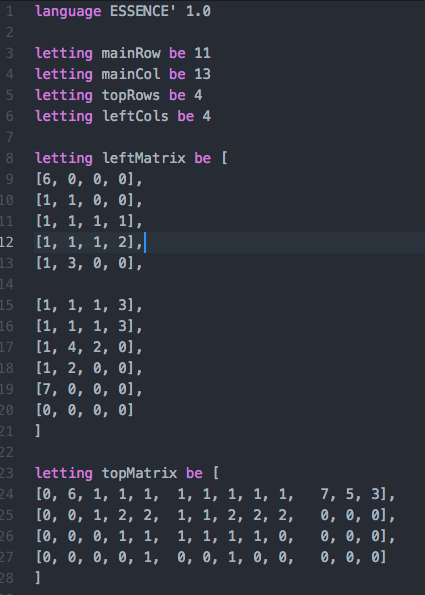
\includegraphics[scale=.6]{param_file_template}
	\caption{Parameter file format example}
	\label{fig:parameter}
\end{figure}


% \begin{figure}[tb]
% 	\centering
% 	\includegraphics[]{}
% 	\caption{Caption here}
% 	\label{fig:figure1}
% \end{figure}

%----------------------------------------------------------------------------------------
%  SECTION : CONSTRAINT PROGRAMMING
% %----------------------------------------------------------------------------------------
% \section{Constraint Programming}
% \label{sec:subsec_cp}

% text


%----------------------------------------------------------------------------------------
%   SUBSECTION: 
%----------------------------------------------------------------------------------------
% \subsection{Subsection}
% \label{subsec:subsec01}

% Begins a subsection.